\documentclass{article}
\usepackage[utf8]{inputenc}
\usepackage{geometry}
\geometry{a4paper, top=2.5cm, bottom=2.5cm, left=3cm, right=3cm, bindingoffset=5mm}
\usepackage[table]{xcolor}

\usepackage{colortbl}
 
\usepackage{multicol}
\usepackage{hyperref}
\usepackage{capt-of}
\usepackage{url}
\usepackage{graphicx}
\usepackage[italian]{babel}
\usepackage[suftesi]{frontespizio}


\title{Relazione di Laboratorio: Esperimento di Millikan}

\author{Gruppo VE\_2:\\ \\Federico Greco C.M 969073\\federico.greco2@studenti.unimi.it\\ \\ Nicolò Favagrossa C.M. 969124\\nicolo.favagrossa@studenti.unimi.it\\ \\Daniele Hasou C.M. 967555\\daniele.hasou@studenti.unimi.it\\ \\ Esperimento eseguito da: Nicolò Favagrossa e Daniele Hasou}
\date{\today\\A.A. 2021-2022}

\begin{document}
\maketitle
\newpage
\tableofcontents
\newpage
\section{Introduzione}
L'esperienza di Millikan, condotta nel 1909 dal fisico statunitense, è un esperimento volto alla misura della carica dell'elettrone. Misurando i tempi di caduta di particelle d'olio ionizzate, infati, lo scienziato era riuscito a misurare con estrema precisione il valore della carica fondamentale, vincendo così il premio Nobel nel 1923 per i suoi studi sull'elettrone. 

In laboratorio l'esperienza consiste nell'introdurre all'interno della camera di Millikan, attraverso un nebulizzatore, delle gocce d'olio che per strofinio si caricano elettricamente. Le particelle d'olio, all'interno della camera, sottoposte alla forza di gravità e alla forza di attrito viscoso dell'aria, cadono verso il basso con una velocità costante: misurando la velocità di caduta è possibile calcolare il raggio della goccia d'olio. Successivamente si itera il procedimento applicando una differenza di potenziale, prima in un verso e poi nell'altro, per calcolare l'effettiva carica presente sulla goccia. Nell'immagine (\ref{Esperienza}) si può osservare un modello schematico dell'esperimento.\footnote{Fonte: \url{https://en.wikipedia.org/wiki/Oil_drop_experiment}}.

A esperienza conclusa, essendo la carica dell'elettrone una quantità nota, si può eseguire un confronto diretto e stimare quantitativamente la coerenza dei dati raccolti.
\begin{figure}[htp!]
\centering
  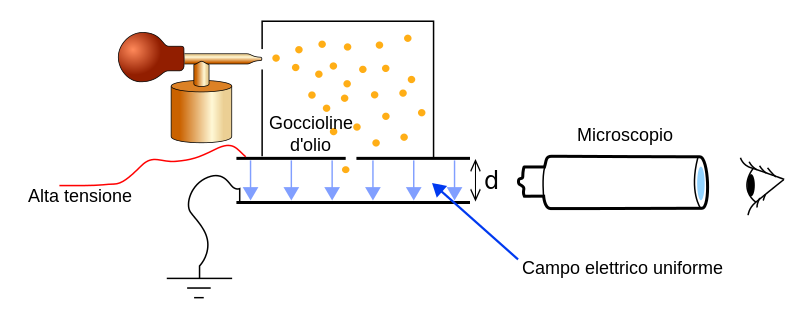
\includegraphics[width= 15cm, height= 7cm]{Schema.png}\\
  \caption{Un semplice schema per presentare visivamente l'esperienza. Le gocce d'olio, introdotte dentro la camera di Millikan mediante un nebulizzatore, si smistano in base alla dimensione entrando, da un foro, nel campo visivo del microscopio tra i due elettrodi. In questo modo si può inziare a misurare, indirettamente, la velocità della goccia d'olio. }
  \label{Esperienza}
\end{figure}
\newpage
\section{Trattazione teorica}
Le goccie d'olio si caricano per strofinio durante la fase di nebulizzazione e all'interno della camera di Millikan, sotto l'effetto dell'accelerazione gravitazionale cadono verso il basso con una velocità di caduta che viene considerata costante ("velocità limite", che viene raggiunta in tempi trascurabili). In caduta libera, la goccia è sottoposta a tre diverse forze la cui somma dei moduli è uguale a zero: la forza peso $\vec{F_p}$, l'attrito viscoso douvuto all'aria $\vec{F_V}$(Legge di Stokes) e la forza di Archimede $\vec{F_A}$.
\begin{equation}
    \sum{\vec{F}} = \vec{F_p}+\vec{F_V}+\vec{F_A}= 0
    \label{sum}
\end{equation}
Impostando la seconda legge di Newton si arriva alla seguente equazione:
\begin{equation}
    \frac{4}{3}\pi r_0^{3}g(\rho_{olio}-\rho_{aria})=6\pi r_0\eta v_r
    \label{NII}
\end{equation}
Dove $r_0$ è il raggio della goccia d'olio che è stata approssimata ad una sfera, $g$ rappresenta l'accelerazione di gravità, $\rho$ la densità, $\eta$ il coefficiente di viscosità e $v_r$ la velocità di regime.
Il valore del coefficienre di viscosità $\eta$ varia in funzione della temperatura: si ha infatti

\begin{equation}
    \eta(T)=[1.800+4.765\times 10^{-3}(T-15^{\circ} C)]\times 10^{-5} Nsm^{-2},
    \label{eta}
\end{equation}
dove T rappresenta la temperatura all'interno della camera di Millikan espressa in gradi centigradi.\\\
Oltre a questo è necessario correggere ulteriormente il coefficiente $\eta$ perchè le dimensioni delle gocce d'olio sono confrontabili con il libero cammino medio delle molecole dell'aria, contraddicendo così una delle ipotesi necessarie per la legge di Stokes, cioè che il mezzo sia omogeneo rispetto all'oggetto che lo attraversa. Applicando questa correzione il coefficiente di viscosità $\eta$ lo si esprime come $\eta_{eff}$:
\begin{equation}
    \eta_{eff}(T,r_0)=\eta(T)\cdot \frac{1}{1+b/(pr_0)}
    \label{eff}
\end{equation}
Dove $b = 8.2 \times 10^{-3} Pa\,m$ è un parametro empirico e $p = 101325 \ Pa$ è la pressione atmosferica.

Sostituento $\eta$ con $\eta_{eff}$ e mettendo a sistema le equazioni (\ref{NII}) e (\ref{eff}) si ottiene un'equazione di secondo grado con soluzione:
\begin{equation}
    r_0=\sqrt{\left(\frac{b}{2p}\right)^2+\frac{9\eta v_r}{2g(\rho_{olio}-\rho_{aria})}}-\frac{b}{2p}
    \label{raggio}
\end{equation}

Attraverso il raggio è ora possibile calcolare la carica dell'elettrone aggiungendo all'equazione (\ref{NII}) la forza associata al campo elettrico:
\begin{equation}
    \frac{4}{3}\pi r_0^{3}g(\rho_{olio}-\rho_{aria})\pm 6\pi r_0 \eta_{eff} v_E\pm qE=0
    \label{Campo}
\end{equation}
Dove $q$ è la carica elettrica dell'elettrone, $v_E$ è la velocità in presenza del campo elettrico ed $E$ è il campo elettrico che si misura attraverso il rapporto tra la differenza di potenziale e la distranza tra le armature $|E|=\Delta V/d$

Attraverso alcuni passaggi algebrici si ricava $q$:
\begin{equation}
    q = -\frac{4}{3}\pi r^3(\rho_{olio}-\rho_{aria})\frac{g}{E} \left(1 \pm \frac{|v_E|}{v_r} \right)
    \label{formula carica}
\end{equation}
L'espressione è da considerarsi col segno (+) se $v_E <0$ e $v_E$ è diretta verso l'alto, col segno  (-) se $v_E>0$ e $v_E$ è diretta verso il basso; imponendo come sistema di riferimento l'asse diretto nella stessa direzione della forza peso.
\newpage
\section{Apparato sperimentale e materiali}
Il setup sperimentale (\ref{Setup Sperimentale}) è diviso in due parti: i materiali e l'apparato di Millikan. I materiali utilizzati durante l'esperienza sono:
\begin{multicols}{2}
\begin{itemize}
    \item Cronometro;
    \item micrometro analogico;
    \item generatore di tensione;
    \item multimetro digitale;
    \item supporto regolabile;
    \item cavi;
    \item nebulizzatore;
    \item fazzoletti;
    \item alcool etilico;
    \item alcool isopropilico.
\end{itemize}
\end{multicols}
\begin{figure}[htp!]
\centering
  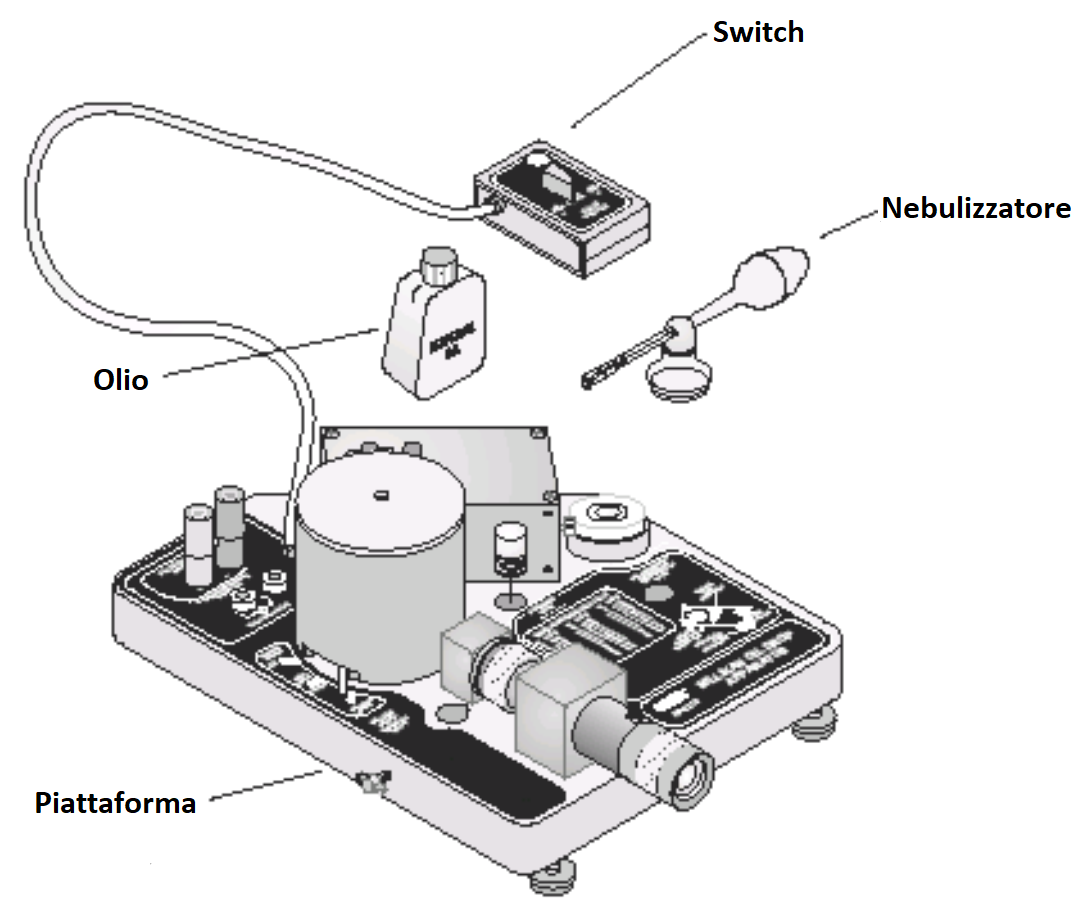
\includegraphics[width=8cm]{Setup sperimentale.png}\\
  \caption{In questa immagine si può osservare come si presenta l'apparato sperimentale in laboratorio. Sono presenti il nebulizzatore, lo switch, l'olio e la piattaforma in cui avviene l'esperimento.}
  \label{Setup Sperimentale}
\end{figure}

Di seguito una breve descrizione:
\begin{itemize}

\item il cronometro è stato utilizzato per misurare in modo diretto il tempo che ogni goccia d'olio impiegava ad attraversare il reticolo, con una sensibilità di $10 \ ms$. 

\item Il micrometro analogico è stato usato per misurare lo spessore del  distanziale posto tra i due elettrodi, con una sensibilità di $0.01 \ mm$ e una portata di $25 \ mm$. 

\item Il generatore di tensione è stato collegato all'apparato tramite dei cavi protetti per produrre il campo elettrico applicando una differenza di potenziale fino a un massimo di $500 \ V$. 

\item Per misurare la temperatura all'interno del laboratorio è stato necessarario un multimetro digitale in grado di misurare la resistenza ($M\Omega$) del termistore presente nell'apparato di Millikan. Così facendo con una  tabella è stato possibile ottenere la temperatura e di conseguenza ricavare il coefficiente $\eta_{eff}$ attraverso le formule (\ref{eta}) e (\ref{eff}). Il multimetro digitale nella modalità resistenza ha una sensibilità di $0.001 \ M\Omega$. 

\item A sostenere l'apparato di Millikan è presente un supporto regolabile attraverso tre manopole per aggiustare l'altezza e l'orientamento del sistema. 

\item Per spruzzare l'olio all'interno della camera è stato usato un nebulizzatore. 

\item Per pulire la configurazione sperimentale sono stati usati dei fazzoletti, alcool etilico e isopropilico: il primo utilizzato per pulire il banco di lavoro e gli oggetti toccati, il secondo per pulire le ottiche.
\end{itemize}
L'apparato di Millikan, rappresentato dall'immagine (\ref{Apparato}) è composto da: un microscopio dotato di due regolazioni che consentono di mettere a fuoco le gocce d'olio e il reticolo all'interno della camera (grazie anche all'ausilio di un ago). Il reticolo consente di misurare la distanza percorsa dalla goccia d'olio; consiste in un quadrato di $3 \ mm$ di lato, suddiviso in quadratini di lato $0.5\ mm$ . La camera è illuminata da una sorgente di luce alimentata da una presa esterna. All'interno dell'apparato è anche possibile trovare una bolla per regolare il piedistallo in modo tale che sia parallelo al terreno. Collegato all'apparato c'è uno switch che permette di eliminare o variare il verso del campo elettrico.
\begin{figure}[htp!]
\centering
  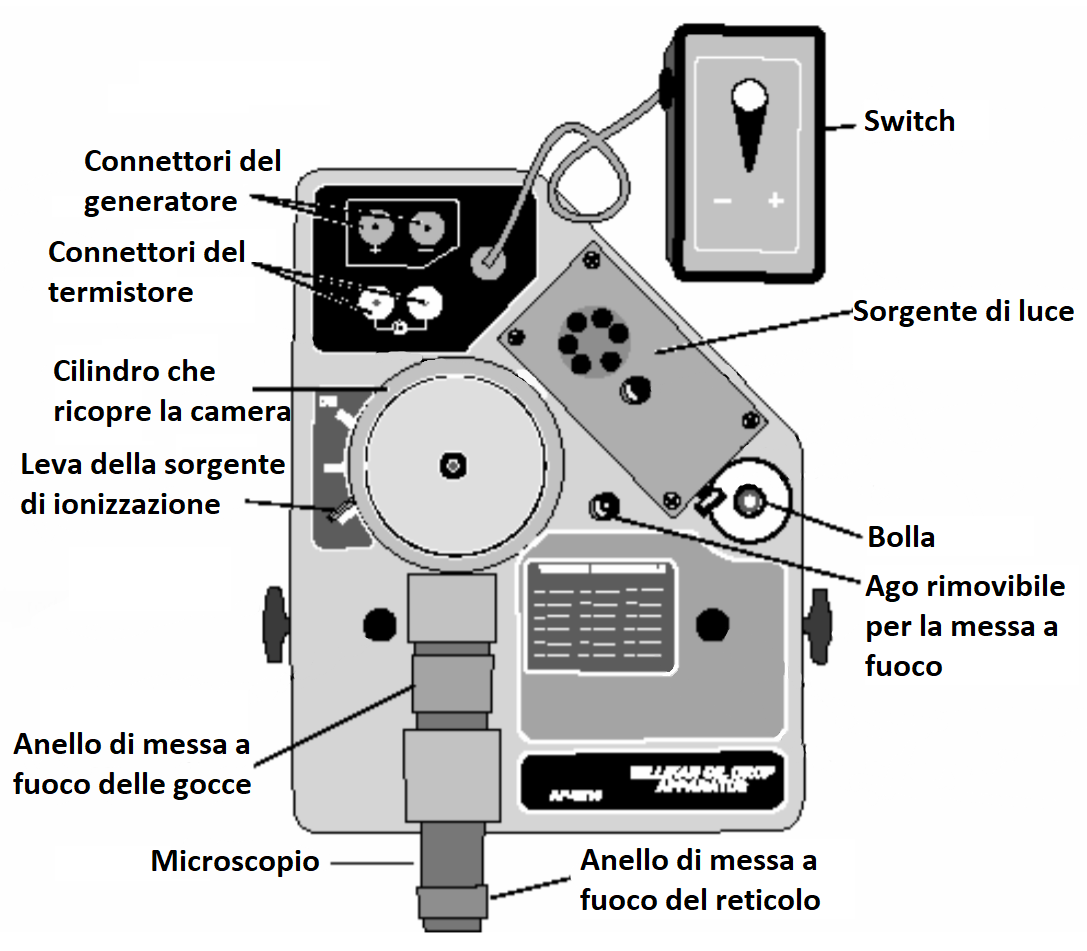
\includegraphics[width=8cm]{Apparato di Millikan.png}\\
  \caption{In questo schema si possono osservare le varie componenti della piattaforma in cui avviene l'esperimento e su cui è posta la camera di Millikan. }
  \label{Apparato}
\end{figure}

La camera di Millikan, schematizzata nell'immagine (\ref{Camera}), partendo dalla base è formata da: una sorgente ionizzante di thorium-232 che serve a caricare le gocce d'olio in caso di debole interazione con il campo elettrico, un elettrodo saldato alla piattaforma, un distanziale che serve a imporre una distanza fissa tra le due armature, il secondo elettrodo fissato con un peso, un cappuccio di plastica forato che ha lo scopo di fare passare solo le gocce vaporizzate e quindi sospese in aria. Per isolare il tutto c'è un cilindro che ricopre l'intera camera con un due fori ai lati facendo entrare la luce della sorgente, da una parte, e visualizzare l'interno della camera con il microscopio dall'altra. Infine il cilindro è chiuso da un disco di plastica forato in cui è possibile spruzzare l'olio.
\begin{figure}[htp!]
\centering
  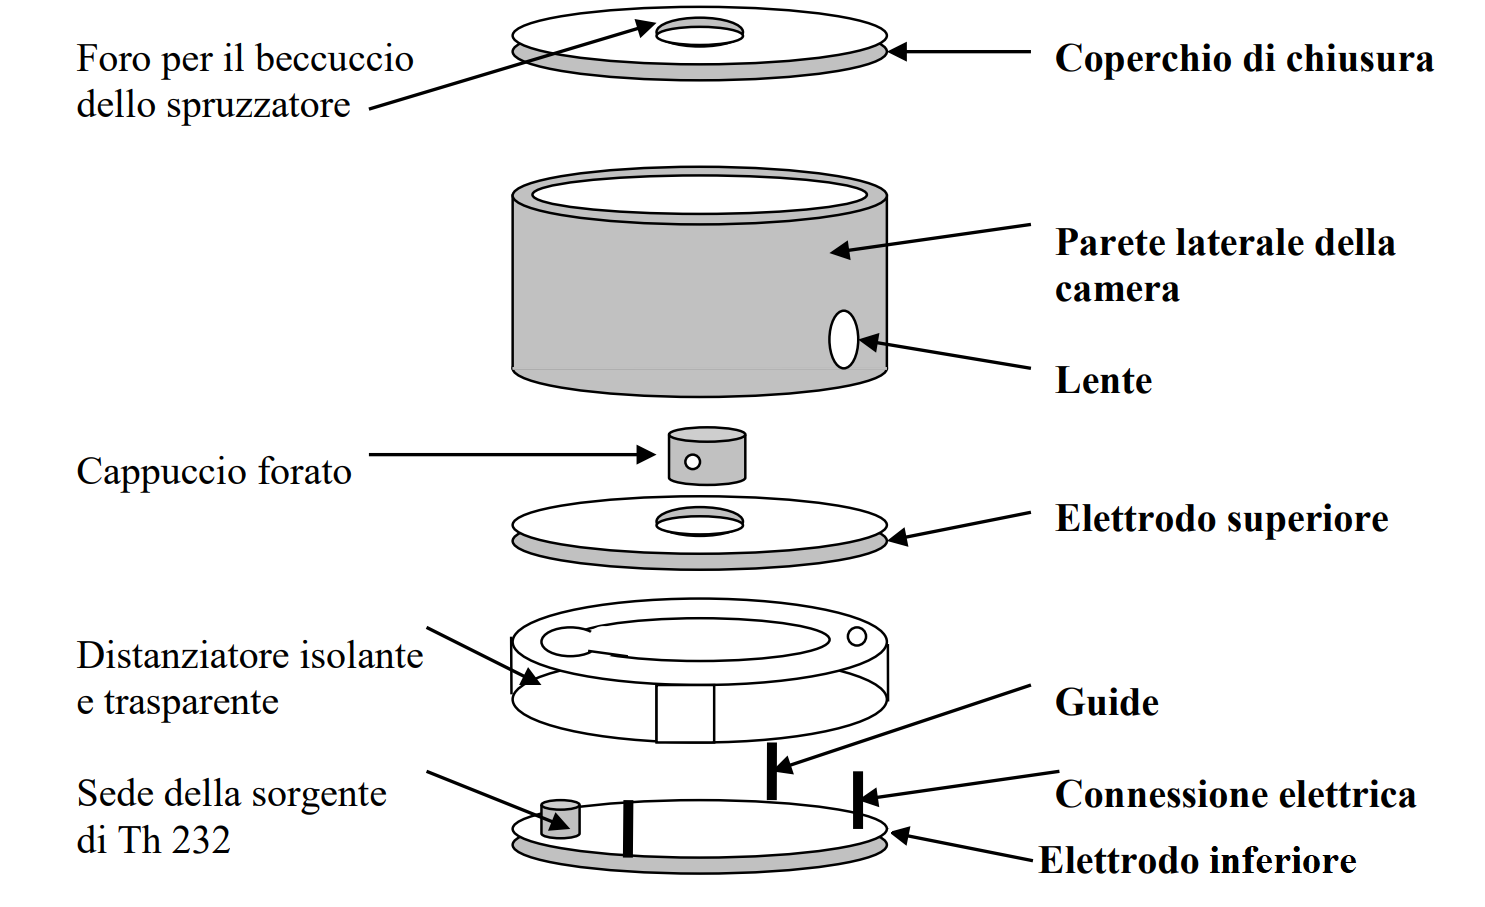
\includegraphics[width=8cm]{Camera di Millikan.png}\\
  \caption{Nella seguente immagine è presente la camera di Millikan in esplosione mettendo in risalto ogni componente. }
  \label{Camera}
\end{figure}
\section{Procedura sperimentale}
\subsection{Preparazione della strumentazione}

Prima di montare l'apparato di Millikan, è stato misurato lo spessore del distanziatore isolante, in modo da conoscere la distanza tra le lastre cariche e dunque il campo elettrico presente all'interno della camera. Per far ciò, è stato misurato lo spessore in diversi punti dell'apparecchio, e si sono calcolate la media e la relativa incertezza. 

Affinchè la velocità misurata grazie al reticolo corrispondesse alla velocità reale, ci si è assicurati che la camera di millikan fosse in bolla, e dunque il suo asse perfettamente parallelo alla forza di gravità. 

Dopodichè, ci si è occupati della messa a fuoco sia del reticolo che dell'interno della camera: per far ciò, nel montare la camera la prima volta, invece del cappuccio forato, è stato utilizzato un ago, in grado di passare attraverso il foro praticato nella piastra superiore. Accendendo la lampada, in grado di illuminare l'interno della camera e di mostrarla all'osservatore attraverso la lente,  è stato dunque possibile mettere a fuoco sia l'ago (posto nella posizione da cui sarebbero entrate le goccioline di olio) che il reticolo, usando i due diversi anelli sul microscopio indicati nell'imagine (\ref{Apparato}).

Una volta assicurate la bolla e la messa a fuoco, è stato possibile estrarre l'ago, riponendolo con cura nella sua sede, ed inserire il cappuccio forato al suo posto, richiudendo poi col coperchio l'intera camera.
\subsection{Metodo di raccolta dati}
Prima di ogni misurazione è stata registrata la resistenza del termistore, in modo da poter stabilire la temperatura all'interno della camera e poter così calcolare la $\eta_{eff}$ da usare nella formula (\ref{raggio}). La tabella per la conversione è nell'appendice (\ref{Conversione}). \`E  stata inoltre scelta e riportata la differenza di potenziale $\Delta V$ tra le armature per il calcolo del campo elettrico.

Usando il nebulizzatore contenente l'olio, si è prima verificato che questa non producesse spruzzi d'aria, poi si è spruzzato l'olio dentro al foro nel coperchio di chiusura, tenendo aperta la leva centrale. Dopo aver verificato un corretto accesso delle goccioline d'olio all'interno della camera, è stata azionata la sorgente di torio, di modo che le particelle ricevessere un'ulteriore fonte di ionizzazione oltre al semplice sfregamento. Passata una decina di secondi, la sorgente è stata richiusa e si è cominciato ad osservare il comportamento delle goccie sul reticolo. In particolare, si è oservato come le varie goccioline si comportavano al variare del campo elettrico nelle tre possibili combinazioni( $E=0$ , $E<0$ , $E>0$), assicurandosi di trovare alcune goccie che si muovesserero in tutti e tre i casi di moto rettilineo uniforme. 

Identificata una particella adatta, sono state misurate le velocità di caduta libera, di caduta e di salita in presenza di campo elettrico, calcolando il tempo di percorrenza di una tacca del reticolo ($\Delta z=0,5\ mm$).

Dalla velocità di caduta libera, è stato possibile ricavare il raggio della particella; dalle due velocità in presenza di campo elettrico si è invece calcolata la carica in essa contenuta.


Finite le prese misure relative ad una singola particella, è stato ritenuto opportuno ripulire con alcool sia la lente che il cappuccio forato: il primo per disinfettare per l'osservatore successivo, il secondo perchè non si accumulasse uno strato d'olio nel forellino, evitando così che lo spruzzo seguente non producesse alcuna particella significativa. Prima di smontare la camera di Millikan, è stato necessario spegnere ogni volta il generatore di potenziale elettrico tra le piaste evitare problematiche legate all'alta tensione. 
\newpage
\section{Analisi dei dati}

Le prime misurazioni effettuate sono stati gli spessori del distanziatore nei diversi punti della corona circolare: in tabella si ritrovano i valori così ottenuti, assieme alla media degli stessi e alla deviazione standard della media. \\
\begin{table}[h!]
    \centering
    \begin{tabular}{|c|c|c|c|c|c||c||c|}
    \hline
    \multicolumn{6}{|c||}{spessore d del distanziatore  [mm]} & $<d>$ [mm] & $\sigma_d$ [mm]\\
    \hline
        7.57 & 7.61 & 7.58 & 7.58 & 7.58 & 7.60 & %\cellcolor{cyan} 
        7.59 & %\cellcolor{cyan} 
        0.01 \\
        \hline


    
    \end{tabular}
    \label{misure d}
    \caption{La tabella mostra i valori dello spessore del distanziatore in diversi punti della circonferenza, la media di tali misure e la deviazione standard della media. }
    \label{tab:my_label}
\end{table} \\
I valori delle velocità di caduta libera e di caduta o salita in presenza di campo elettrico sono stati invece registrati nella tabella presente nell'appendice A, accanto al valore della carica nella particella calcolata usando le formule (\ref{formula carica}).
Per ogni singola goccia d'olio sono state effettuate dieci misure della carica presente al suo interno utilizzando il procedimento descritto nel sezione (4): cinque per ogni verso del campo elettrico. In questo modo, si è cercato di acquisire un numero di dati significativo, evitando allo stesso tempo che misure ottenute in maniera errata avessero un peso eccessivo nel calcolo finale. Infatti dopo numerose misure effettuate sulla stessa goccia si osservava una diversa interazione con il campo elettrico.\\ In particolare questo fenomeno veniva riscontrato quando la goccia selezionata urtava una delle numerose gocce in sospensione dentro la camera di Millikan. In queste situazioni, la velocità della goccia variava, rendendo la singola misura compromessa: si è scelto di annullare la misura proseguendo le successive misure con la medesima goccia dopo aver controllato che il suo moto fosse rimasto regolare.
Le misure di carica così ottenute sono state riordinate in odine crescente, e riportate nella tabella sottostante. \\ 
\begin{table}[h!]
    

\begin{center}
\begin{tabular}{ |c|c|c|c|c|c| } 
\hline
\multicolumn{6}{|c|}{Cariche contenute nelle particelle d'olio [C]} \\
 \hline
 
 1.15181E-19 &	1.99695E-19	& 2.14775E-19 &	5.1947E-19 &	6.34608E-19 &	9.83437E-19 \\
 \hline
1.37782E-19	& 2.06472E-19 & 2.19402E-19 &	5.75069E-19 &	6.58909E-19 &	1.01662E-18 \\
\hline
1.40077E-19	& 2.08197E-19 &	2.21438E-19 &	5.85656E-19 &	6.71084E-19 &	1.03202E-18 \\
\hline
1.41481E-19	& 2.08932E-19 &	2.25023E-19 &	5.89224E-19 &	6.72701E-19 &	1.03342E-18 \\
\hline
1.55889E-19	& 2.10500E-19 &	2.27274E-19 &	5.90269E-19 &	6.86477E-19 &	1.03507E-18 \\
\hline
1.87817E-19	& 2.10971E-19 &	2.28275E-19 &  6.1146E-19 &	7.11761E-19 &	1.06616E-18 \\
\hline
1.88995E-19	& 2.13396E-19 &	2.32447E-19 &	6.14777E-19 &	7.57804E-19 &	1.07214E-18 \\
\hline
1.92962E-19	& 2.14451E-19 &	4.60990E-19 &	6.18816E-19 &	8.79731E-19 &	1.09232E-18 \\
\hline
1.97664E-19	& 2.14705E-19 &	4.71306E-19 & 6.21833E-19 &	9.08328E-19	& \\

 
 \hline

\end{tabular}
 \label{cariche misurate}
\caption{la tabella contiene i valori delle cariche contenute nelle diverse particelle d'olio, oridinate in ordine crescente.}
\label{table:1}
\end{center}
\end{table} \\
Per valutare quale sia il valore della carica elementare che meglio si adatta ai valori ottenuti, è stata determinata la quantità
\begin{equation}
    S(q)=\sum_{i=1}^{N}[\frac{Q_i}{k_i(q)}-q]^2
    \label{S(q)}
\end{equation}
dove N indica il numero di cariche ottenute, $Q_i$ rappresenta la carica i-esima , $q$ è la variabile che permette di studiare il valore della carica fondamentale, e $k_i(q)$ il valore che si ottinene calcolando la parte intera dell'espressione $\frac{Q_i}{q}+0.5$, ovvero il numero intero diverso da zero che più si avvicina al rapporto $\frac{Q_i}{q}$ .

La carica  $q*$ che rende minima la quantità $S(q)$ rappresenta il valore che con maggiore probabilità viene assunto dalla carica elementare. $S(q)$ non è una funzione derivabile nel suo dominio, ma esiste un intervallo nell'intorno di $q*$ in cui i vari $k_i$ rimangono costanti, e pertanto $S(q)$ diventa una funzione regolare e derivabile. Per individuare l'intorno del punto di minimo, è stato tracciato il grafico campionando in maniera fitta vari valori di $q$, ottenendo il grafico (\ref{Cariche}) a pagina seguente.
\begin{figure}[h!]
\centering
  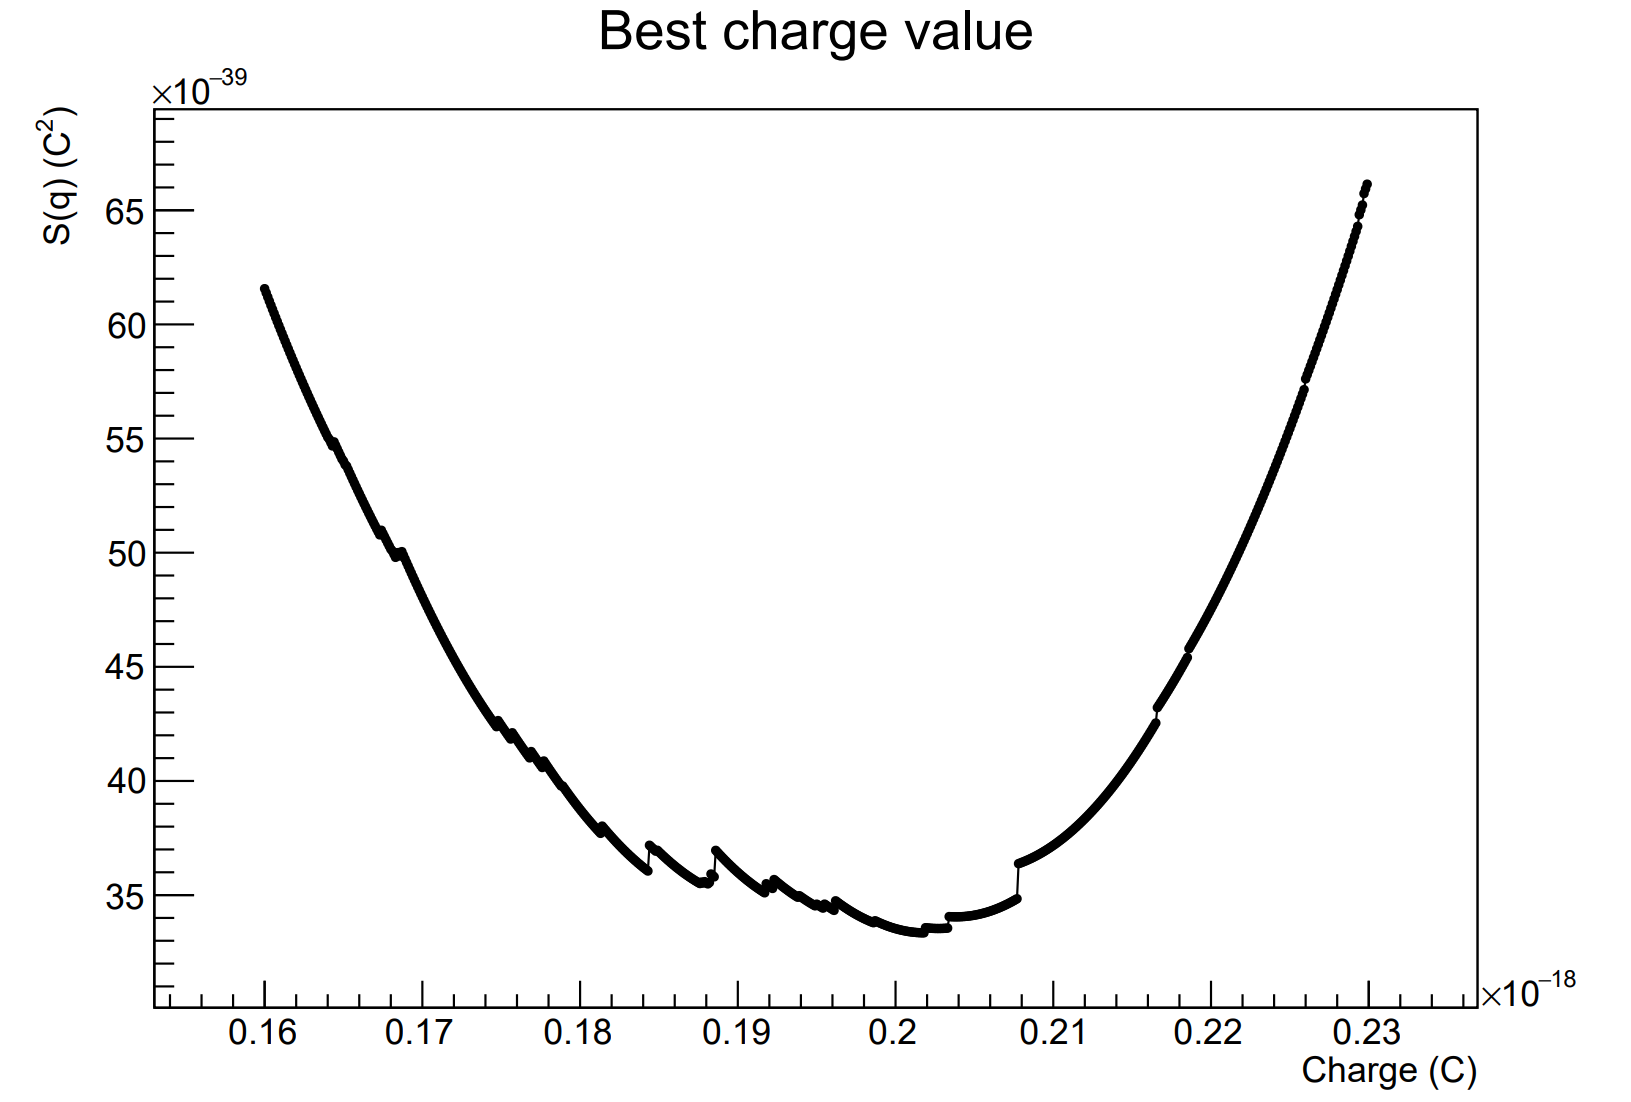
\includegraphics[width=12cm]{Cariche.png}\\
  \caption{Il grafico rappresenta la quantità $S(q)$ al variare di $q$. Come si nota, la funzione non è continua, ma il punto di minimo si trova in un intorno di $q=2.0\times10^{-19} C$, dove la funzione è continua e  derivabile. }
  \label{Cariche}
\end{figure}
\newpage Derivando ora la funzione (\ref{S(q)}) si ottiene:
\begin{equation}
    q*=\frac{1}{N}\sum_{i=1}^{N}\frac{Q_i}{k_i}.
    \label{deriv S(q)}
\end{equation}
Per i dati raccolti, si calcola che $q*$ vale $2.02\times10^{-19} \ C$.

L'incertezza relativa al valore della carica fondamentale così ritrovato si calcola come la deviazione standard della media dei valori di $\frac{Q_i}{k_i}$, ovvero:
\begin{equation}
    \sigma_{q*}=\sqrt{\frac{S(q*)}{N(N-1)}}=\sqrt{\frac{3.36\times 10^{-38} C^{2}}{53\times 52}}=3.5\times10^{-21} \ C
\end{equation}\\
Il valore della carica fondamentale così ricavata è dunque
\begin{equation}
    q*=(2.02\pm0.04)\times10^{-19}\ C
\end{equation}
Il valore atteso è di $1.60\times 10^{-19}\ C$. Calcolando la discrepanza tra il risultato teorico e sperimentale si ottiene:
\begin{equation}
    z= \frac{|q_{teo}-q*|}{\sigma_{q*}} > 10
    \label{z}
\end{equation}
Il risultato sperimentale risulta quindi distante dal valore teorico  $10\sigma_{q*}$, molto più grande dell'intervallo di $2\sigma_{q*}$ che è stato scelto come intervallo di accettabilità statistica. Dunque si può affermare che il risultato sperimentale risulta inconsistente rispetto a quello atteso.
\newpage
\section{Conclusione}
Ricapitolando, l'obbiettivo dell'esperienza è misurare la carica dell'elettrone attraverso l'esperimento svolto dal fisico Millikan nei primi anni del Novecento. Si è studiato l'andamento delle gocce d'olio all'interno della camera di Millikan in presenza e assenza di campo elettrico per ricavare prima il raggio e poi la carica delle stesse. 

Il risultato dell'esperienza, in seguito all'analisi dati, è deludente. Infatti il minimo della funzione rappresentata nel grafico (\ref{Cariche}) corrisponde a $q*=(2.02\pm0.04)\times10^{-19}\ C$. Il valore atteso è di $1.60\times 10^{-19}\ C$. La discrepanza tra il risultato sperimentale e il valore teorico corrisponde a: $\Delta = |q_{teo}-q*|=0.42\ C$, che corrisponde a dieci volte la deviazione standard su $q*$, ipotizzando che le misure si distribuiscano secondo una gaussiana si trova l'osservabile $z$, potendo dimostrare quantitativamente l'esito negativo dell'esperienza. Osservando il grafico (\ref{Cariche}), siamo portati a pensare che l'intero esperimento sia soggetto ad un errore sistematico. 

Durante la presa dati abbiamo avuto molte difficoltà nell'individuare le gocce d'olio che rispondessero in maniera appropriata al cambio o all'assenza del campo elettrico. Abbiamo osservato che la maggior parte delle gocce, in assenza di campo elettrico, rimanevano approssimativamente stazionarie rendendo impossibile la misura della velocità in caduta libera. Allo stesso tempo, le gocce che compivano un moto uniforme di caduta libera non sembravano minimamente perturbate dalla presenza del campo elettrico.

Per quanto riguarda i dati che siamo riusciti a prendere, abbiamo notato che il moto delle goccie selezionate risultava disturbato (soprattutto in assenza di campo elettrico) e non continuo. Come causa principale possiamo individuare le dimensioni ridotte delle gocce d'olio che causavano un moto irregolare.
Osservando una velocità irregolare siamo portati a pensare che nel nostro sistema la risultate delle forze non fosse nulla, in contrasto con le ipotesi formulate nella trattazione teorica. Di conseguenza la formula (\ref{formula carica}) non è più valida nel nostro sistema, spiegando così il motivo del fallimento dell'esperienza. Un'altra importante cosiderazione potrebbe riguardare un errore svolto durante le fasi preliminari dell'esperienza, in particolare quando è necessario verificare che l'intero apparato sia in bolla. Se le gocce d'olio non svolgono moti paralleli al reticolo graduato all'interno dell'apparato, l'intera presa dati viene compromessa.
\newpage
\appendix
\section{Misure-dati grezzi}

\begin{table}[h!]
\centering
  \fbox{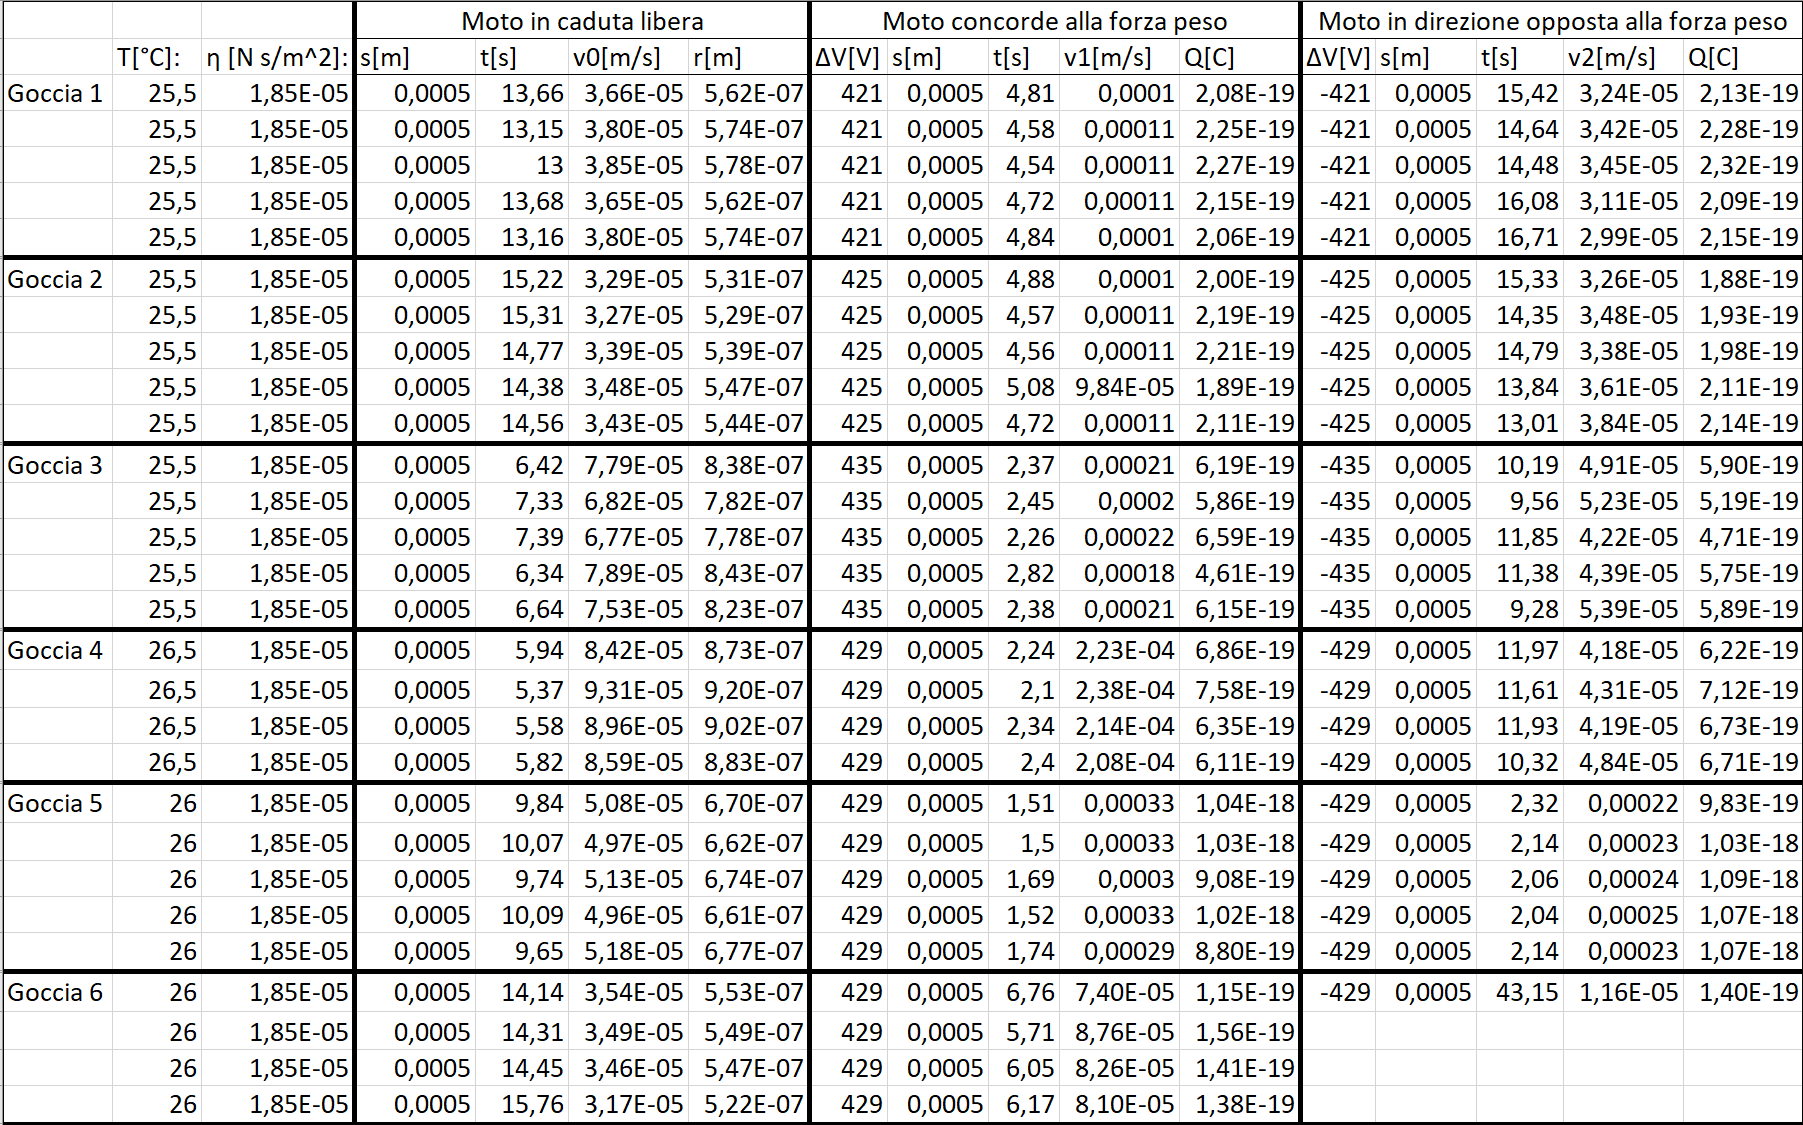
\includegraphics[width=15cm, height=13cm,keepaspectratio]{Dati grezzi.png}}
  \caption{Nella seguente tabella sono stati riportati tutti i dati grezzi presi durante l'esperienza in laboratorio }
  \label{Dati grezzi}
\end{table}

\section{Tabella per la conversione resistenza-temperatura}
\begin{table}[h!]
\centering
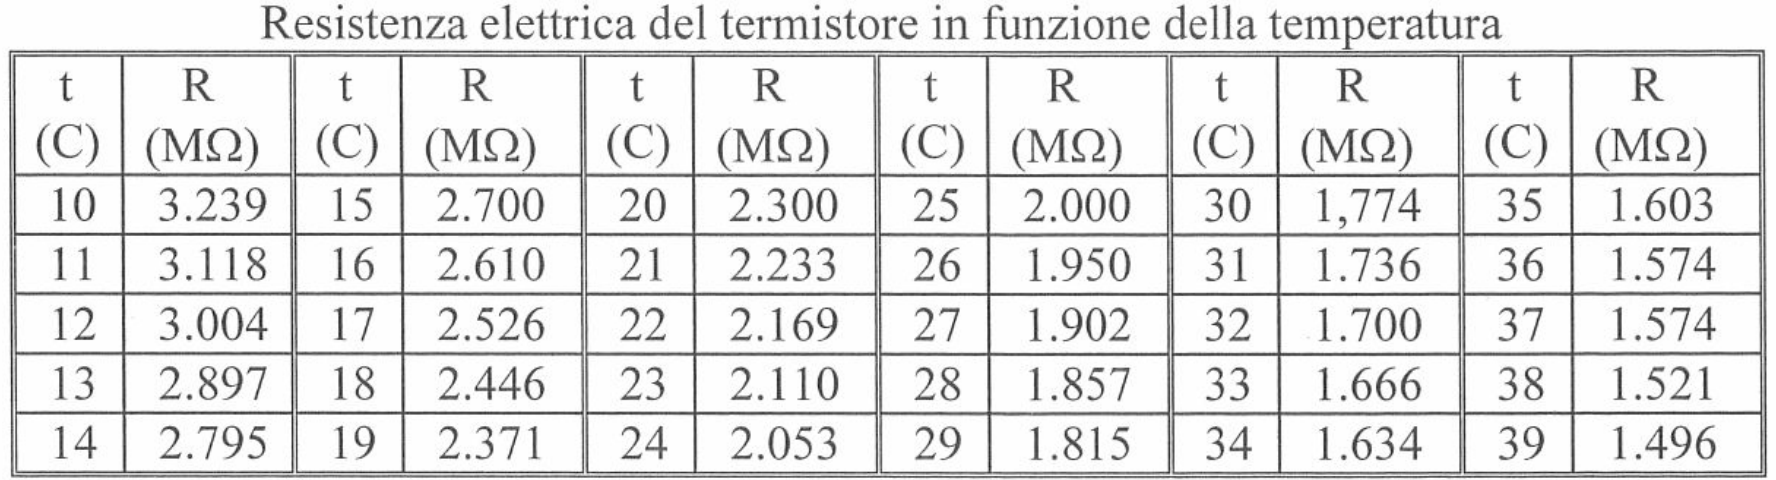
\includegraphics[scale=0.3]{Tabella conversione.png}
  \caption{Attraverso un multimetro si misura la resistenza del termistore, grazie alla seguente tabella è possibile convertire il valore misurato in una temperatura espressa in gradi Celsius all'interno del laboratorio.}
  \label{Conversione}
\end{table}
\end{document}
